\chapter{}
\section{}
In diesem Aufgabenteil soll das Drehzahl-Drehmomentkennlinienfeld der Asynchronmaschine aus dem Versuchsaufbau im Labor Antriebstechnik gemessen werden. Diese wird in der Abbildung 5 dargestellt.
\begin{figure}[h]
	\centering
	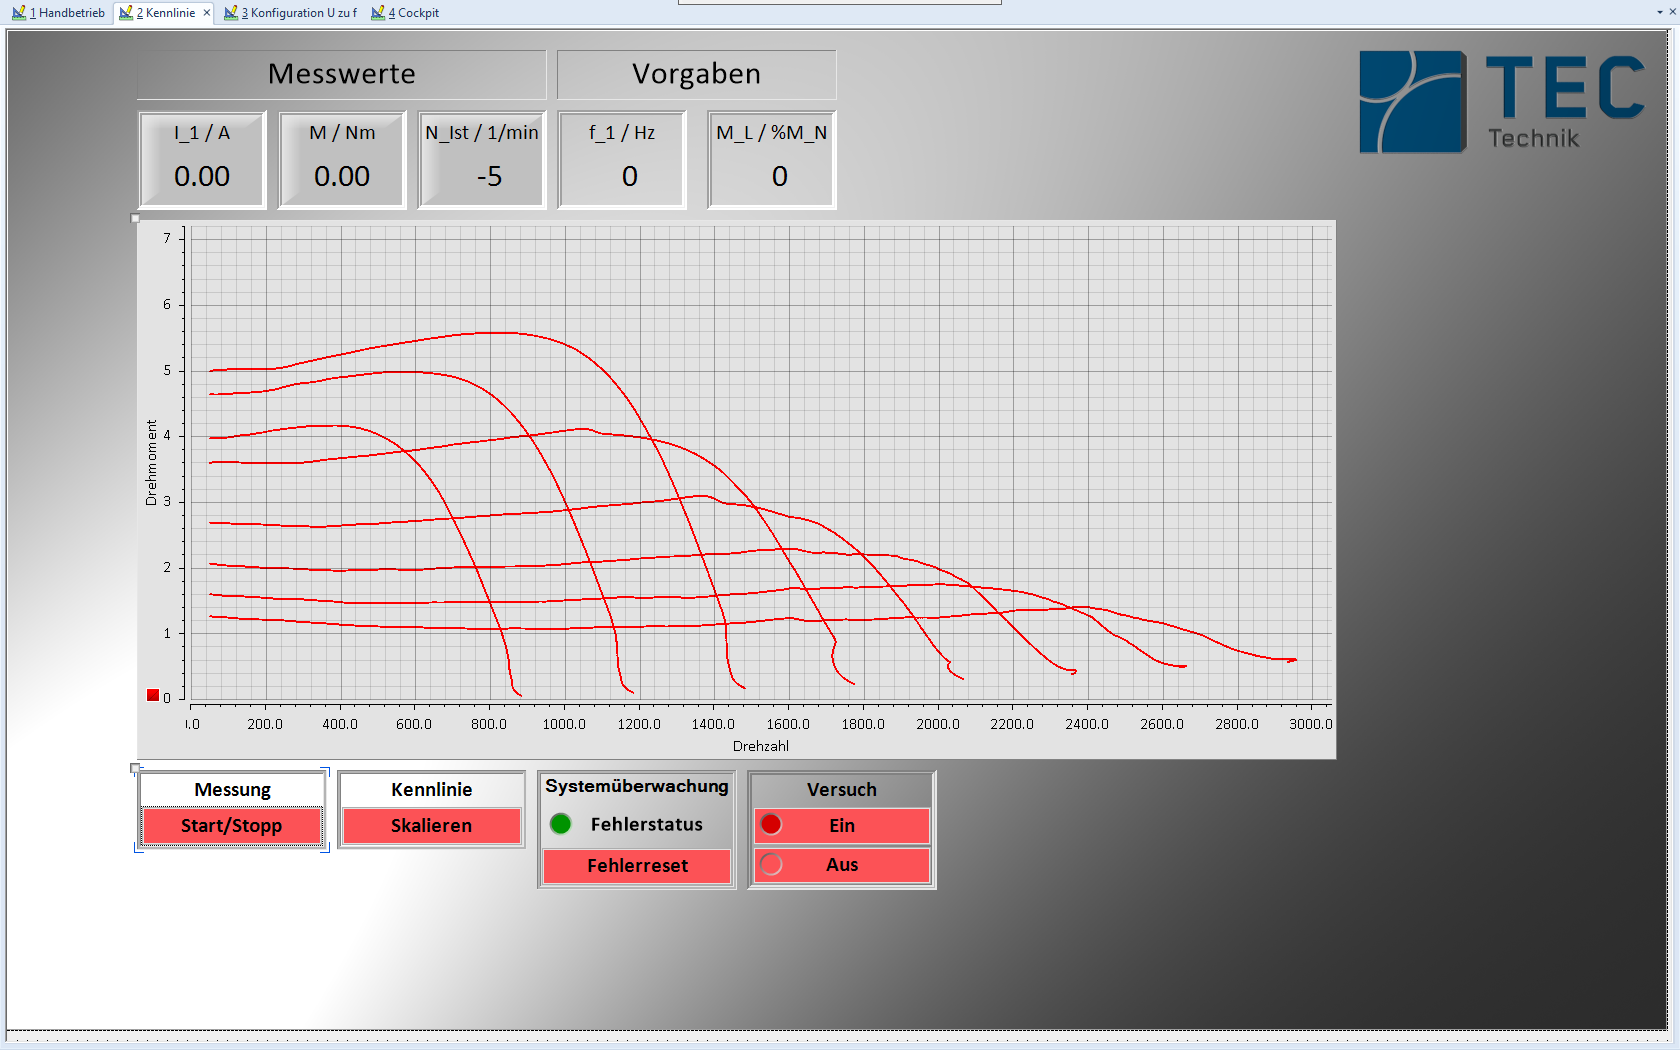
\includegraphics[width=\textwidth]{./Bilder/ele3.png}
	\caption{Drehzahl-Drehmomentkennlinienfeld}
	\label{fig:7a}
\end{figure}

\section{}
Hier wird nun das Kennlinienfeld mit dem Kennlinienfeld aus der Abbildung 6.19 (Skript Elektrische Antriebe) verglichen.\\
Bei geringe Drehzahl $ N $ der Abbildungen zueinander, kann man einen eindeutigen Unterschied erkennen. Dies ist so, weil wir den Idealfall angenommen haben, dass der Statorwiderstand $ R1 = 0\Omega $ sei. Im realen Betrieb ist dies aber nicht der Fall. Der Statorwiderstand hat bei niedrige Statorfrequenzen einen höheren Einfluss auf die Drehmomentkennlinie, da der reale Statorwiderstand für niedrige Statorfrequenzen einen größeren Anteil zur Gesamtimpedanz beiträgt.

\section{}
Im dritten Aufgabenteil soll nun eine Beziehung angegeben werden, wie man bei bekanntem Statorstrombetrag $ I_{1} $ und bekanntem Statorwiderstand $ R_{1} $ der Betrag der Ausgangsspannung $ U_{1} $ verändert werden muss, um dieses Verhalten zu verbessern.

\textbf{???\textit{\underline{???}}}

\section{}
Im letzten Aufgaben Teil haben wir eine erneute Messung mit unseren Anpassung durchgeführt, die wir im dritten Aufgabenteil getroffen haben.\\
In der Abbildung \ref{fig:7d} sieht man nun das Ideale Drehzahl-Drehmomentkennlinienfeld, wo das Drehmoment für kleine Statorfrequenzen kompensiert wurde.
\begin{figure}[h]
	\centering
	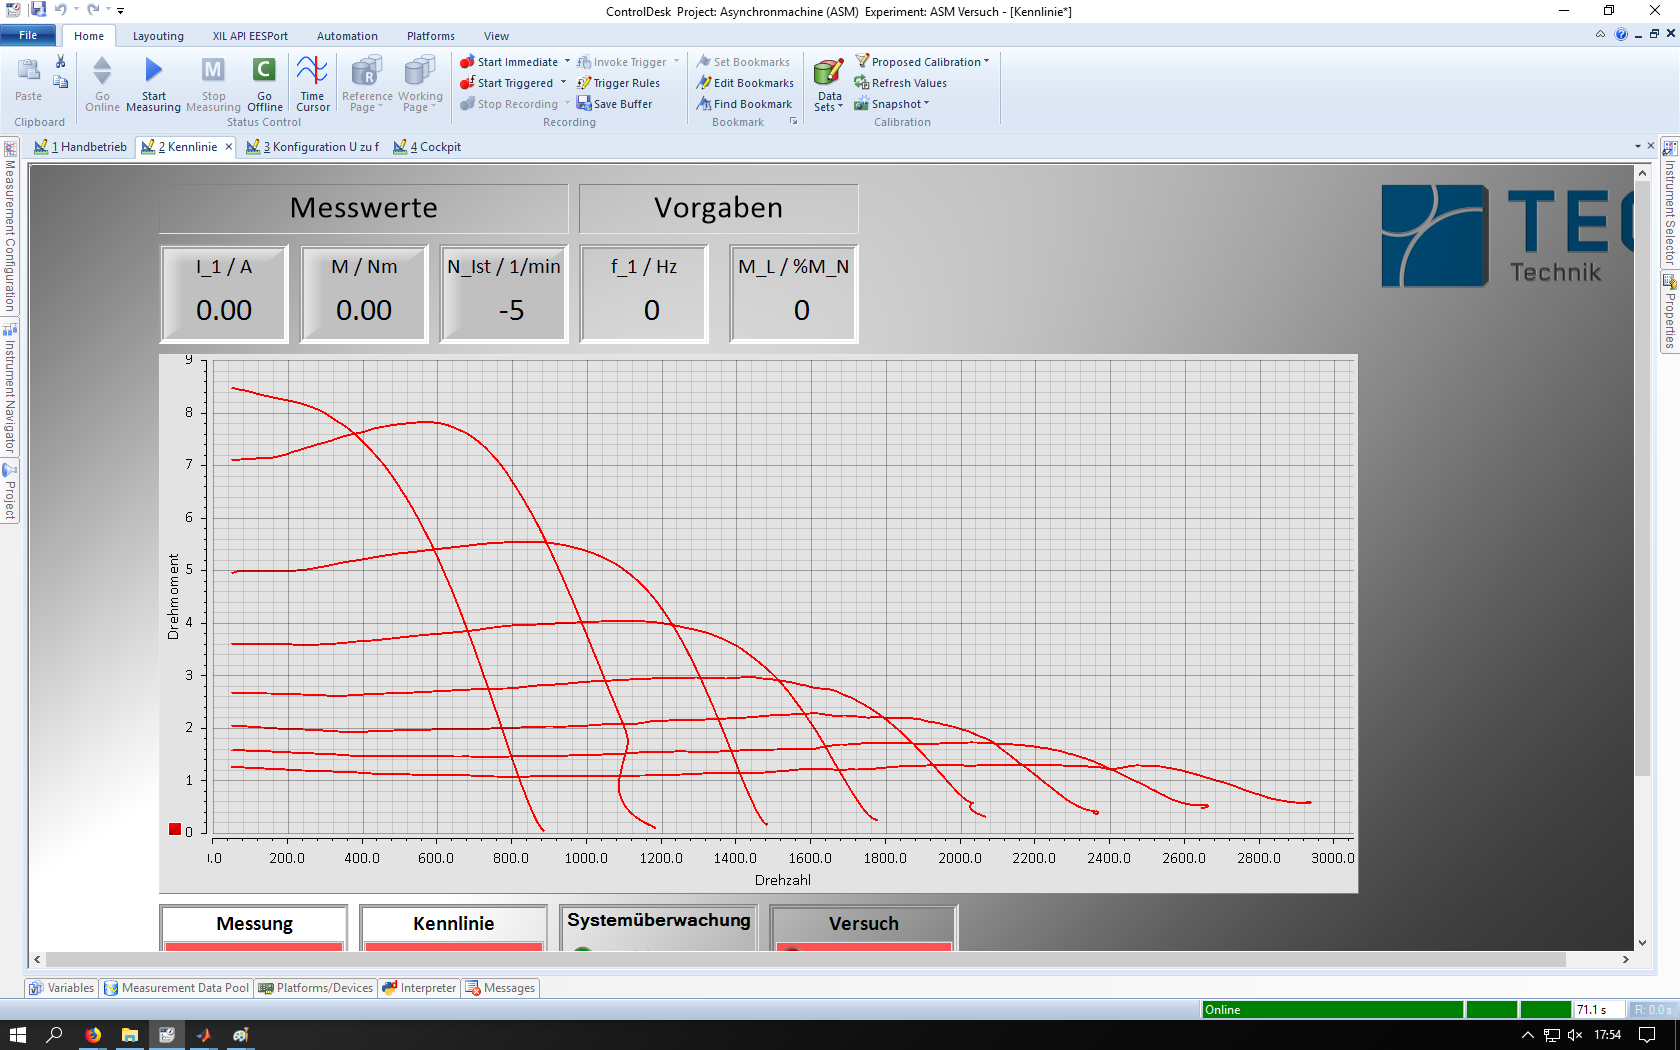
\includegraphics[width=\textwidth]{./Bilder/ele2.png}
	\caption{Drehzahl-Drehmomentkennlinienfeld kompensiert}
	\label{fig:7d}
\end{figure}